\section{Use-case}
\subsection{Lược đồ use-case của hệ thống}

Chi tiết về lược đồ use-case của hệ thống:

\href{https://app.diagrams.net/#G1Myz6UnduM7vZYhCvuX0KpLPWf_OdprEM#%7B%22pageId%22%3A%22aGwoCCFz17a1391KKWEK%22%7D}{Tổng hợp diagram hệ thống BPSky}

\begin{figure}[H]
    \begin{center}
        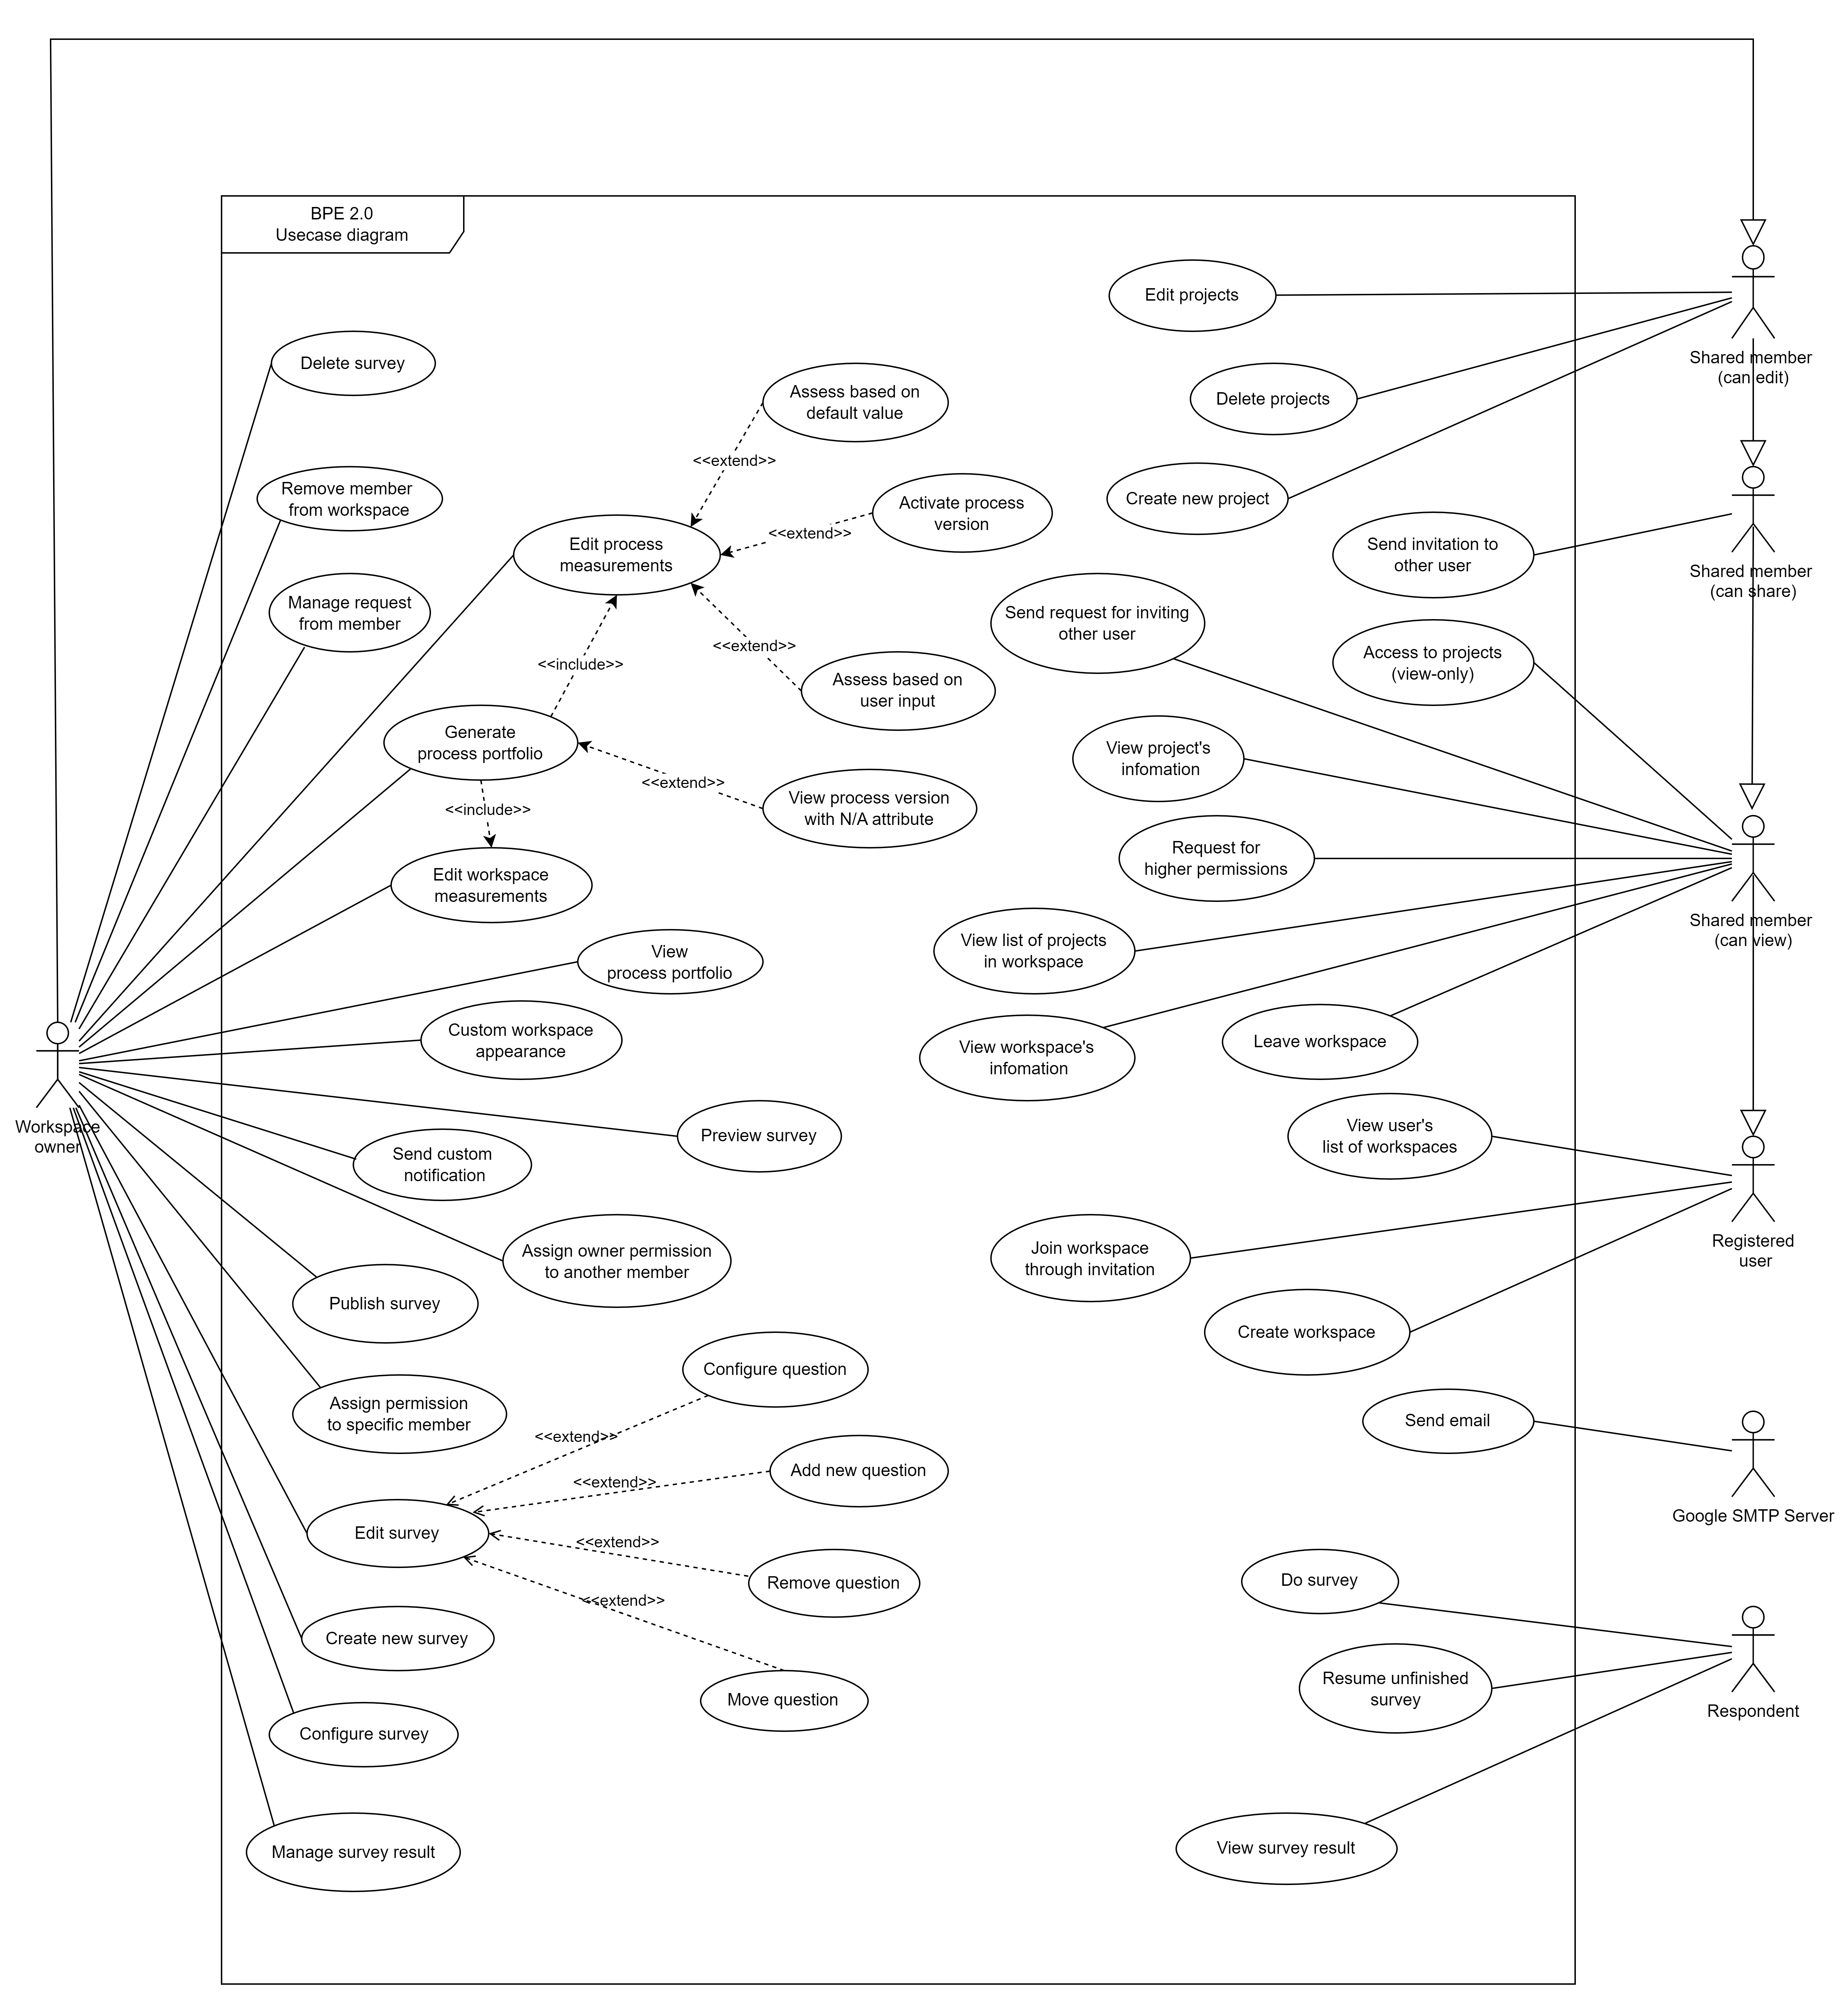
\includegraphics[width=0.85\textwidth]{Content/Phân tích và thiết kế hệ thống/documents/Use case/images/System usecase - HK232.png}
        \vspace{0.5cm}
        \caption{Lược đồ use-case hệ thống}
        \label{fig: Lược đồ use-case hệ thống}
    \end{center}
\end{figure}

% Trang workspace

\subsubsection{Create new workspace}

\begin{table}[H]
\def\arraystretch{2}%
\centering
\resizebox{\textwidth}{!}{%
\begin{tabular}{|p{3cm}|p{11cm}|}
\hline
\textbf{Use-case name}     & Create new workspace
\\ \hline
\textbf{Actor}             & Registered user
\\ \hline
\textbf{Description}       & Người dùng tạo mới workspace
\\ \hline
\textbf{Trigger}           & Không
\\ \hline
\textbf{Pre-conditions}    & Người dùng đã đăng ký vào hệ thống và đăng nhập thành công, hiện tại đang ở giao diện Default homepage
\\ \hline
\textbf{Post-conditions}   & Người dùng tạo mới workspace thành công, và trở thành workspace owner của workspace đó
\\ \hline
\textbf{Normal flow} &
  \begin{enumerate}
      \item Người dùng ở giao diện Default homepage, hiện đang hiển thị danh sách workspace của người dùng đó
      \item Người dùng chọn nút “Create workspace”
      \item Hệ thống mở modal yêu cầu thông tin của workspace: Workspace name, workspace description
      \item Người dùng nhập tên (Name) của workspace
      \item Người dùng nhập mô tả (Description) của workspace
      \item Người dùng chọn nút “Save” để lưu thông tin và hoàn tất tạo mới workspace
  \end{enumerate}
  \\ \hline
\textbf{Alternative flows} & Không
\\ \hline
\textbf{Exceptions} &
  \begin{tabular}{p{10cm}}
      2a. Người dùng chọn nút “Cancel” để đóng modal nhập thông tin workspace
      \\
      3a. Người dùng sử dụng tên của workspace đã tồn tại
      \\ 
      \begin{tabular}{p{9cm}}
          3a.1. Hệ thống yêu cầu người dùng sửa lại tên phù hợp
          \\ 
          3a.2. Tiếp tục bước 4
      \end{tabular}
      \\
      3b. Người dùng không nhập tên của workspace
      \\ 
      \begin{tabular}{p{9cm}}
          3b.1. Hệ thống yêu cầu người dùng phải điền thông tin bắt buộc
          \\ 
          3b.2. Tiếp tục bước 4
      \end{tabular}
  \end{tabular}
  \\ \hline
\end{tabular}
}
\end{table}

\subsubsection{View user’s list of workspaces}

\begin{table}[H]
\def\arraystretch{2}%
\centering
\resizebox{\textwidth}{!}{%
\begin{tabular}{|p{3cm}|p{11cm}|}
\hline
\textbf{Use-case name}     & View user’s list of workspaces
\\ \hline
\textbf{Actor}             & Registered user
\\ \hline
\textbf{Description}       & Xem danh sách những workspaces đã tham gia của người dùng
\\ \hline
\textbf{Trigger}           & Không                                                      \\ \hline
\textbf{Pre-conditions}    & Người dùng đã đăng ký vào hệ thống và đăng nhập thành công \\ \hline
\textbf{Post-conditions}   & Người dùng xem được danh sách những workspaces đã tham gia \\ \hline
\textbf{Normal flow} &
  \begin{enumerate}
      \item Người dùng hiện tại đang ở giao diện Default homepage
      \item Người dùng chọn tab "Recently opened" để xem danh sách những workspace đã tham gia được sắp xếp theo thời gian mở gần nhất
  \end{enumerate}
  \\ \hline
\textbf{Alternative flows} & 2a. Người dùng chọn tab "Pin workspace" để xem danh sách những workspace được ghim
\\ \hline
\textbf{Exceptions}        & Không
\\ \hline
\end{tabular}%
}
\end{table}

\subsubsection{Pin workspace}

\begin{table}[H]
\def\arraystretch{2}%
\centering
\resizebox{\textwidth}{!}{%
\begin{tabular}{|p{3cm}|p{11cm}|}
\hline
\textbf{Use-case name}     & Pin workspace
\\ \hline
\textbf{Actor}             & Registered user
\\ \hline
\textbf{Description}       & Người dùng ghim workspace
\\ \hline
\textbf{Trigger}           & Không
\\ \hline
\textbf{Pre-conditions}    & Người dùng đã đăng ký vào hệ thống và đăng nhập thành công, hiện tại đang ở giao diện Default homepage
\\ \hline
\textbf{Post-conditions}   & Người dùng ghim workspace thành công, và có thể xem những workspace được ghim ở trang Pinned workspace
\\ \hline
\textbf{Normal flow} &
  \begin{enumerate}
      \item Người dùng ở giao diện Default homepage, hiện đang hiển thị danh sách workspace của người dùng đó
      \item Người dùng chọn icon hình ngôi sao ở item workspace tương ứng để ghim workspace
  \end{enumerate}
  \\ \hline
\textbf{Alternative flows} & Không
    2a. Người dùng chọn icon hình ngôi sao ở item workspace tương ứng để bỏ ghim workspace
    \\
    \\ \hline
\textbf{Exceptions} &
    \\ \hline
\end{tabular}
}
\end{table}

\subsubsection{Gửi lời mời đến người dùng khác vào workspace}

\begin{table}[H]
\def\arraystretch{2}%
\centering
\resizebox{\textwidth}{!}{%
\begin{tabular}{|p{3cm}|p{11cm}|}
\hline
\textbf{Use-case name}    & Gửi lời mời đến người dùng khác vào workspace
\\ \hline
\textbf{Actor}            & Thành viên đã tham gia vào workspace
\\ \hline
\textbf{Description}      & Người dùng gửi lời mời tham gia workspace cho người dùng trong hệ thống. 
\\ \hline
\textbf{Trigger}          & Không
\\ \hline
\textbf{Pre-conditions}   & Người dùng đã đăng nhập vào hệ thống thành công
\\ \hline
\textbf{Post-conditions}  & Gửi lời mời người dùng trong hệ thống vào workspace thành công.
\\ \hline
\textbf{Normal Flow} &
    \begin{enumerate}
        \item Người dùng ở giao diện Default homepage, hệ thống hiển thị danh sách những workspace mà người dùng tham gia/sở hữu
        \item Người dùng chọn icon "Menu" ở workspace mà người dùng tham gia với quyền hạn của viewer để hiển thị dropdown menu
        \item Người dùng chọn nút “Share” để hiện modal chia sẻ workspace:
        \begin{enumerate}
            \item Những người hiện có trong workspace
            \item Quyền hạn của những người hiện có trong workspace
        \end{enumerate}
        \item Người dùng nhập email của người được mời để tìm kiếm người dùng trong hệ thống
        \item Người dùng chọn quyền hạn của người dùng được mời vào workspace
        \item Người dùng chọn “Send” để gửi lời mời tới người dùng
    \end{enumerate}
 \\ \hline
\textbf{Alternative flows} &
  \begin{tabular}{p{10cm}}
  4a. Email của người được mời không tồn tại trên hệ thống
    \begin{tabular}{p{9cm}}
          4a.1. Hệ thống hiển thị không tìm thấy kết quả phù hợp
    \end{tabular}
  \\
  5a. Người dùng gán quyền hạn cho người được mời vào workspace vượt quá quyền hạn hiện có trong workspace
      \begin{tabular}{p{9cm}}
          5a.1. Hệ thống thông báo lỗi yêu cầu người dùng gán quyền cho người được mời không vượt quá quyền hạn hiện có (Editor > Sharer > Viewer)
          \\
          5a.2. Tiếp tục ở bước 5
      \end{tabular}
  \\
  \end{tabular} 
\\ \hline
\textbf{Exceptions} &
  \begin{tabular}{p{10cm}}
    5a. Người dùng chọn “Cancel” để hủy yêu cầu và đóng modal
  \end{tabular}
\\ \hline
\end{tabular}%
}
\caption{Use-case scenario cho use-case Gửi lời mời đến người dùng khác vào workspace}
\end{table}

\subsubsection{Gửi yêu cầu mời người dùng khác vào workspace}

\begin{table}[H]
\def\arraystretch{2}%
\centering
\resizebox{\textwidth}{!}{%
\begin{tabular}{|p{3cm}|p{11cm}|}
\hline
\textbf{Use-case name} & Gửi yêu cầu mời người dùng khác vào workspace
\\ \hline
\textbf{Actor} & Workspace member
\\ \hline
\textbf{Description} & Gửi yêu cầu “Chia sẻ workspace đến người khác” tới workspace owner để được xét duyệt
\\ \hline
\textbf{Trigger} & Không 
\\ \hline
\textbf{Pre-conditions} & Người dùng đã đăng ký vào hệ thống và đăng nhập thành công
\\ \hline
\textbf{Post-conditions} & Người dùng gửi thành công yêu cầu “Chia sẻ workspace đến người khác” tới workspace owner để được xét duyệt 
\\ \hline
\textbf{Normal flow} &
  \begin{enumerate}
      \item Người dùng ở giao diện Default homepage, hệ thống hiển thị danh sách những workspace mà người dùng tham gia/sở hữu
      \item Người dùng chọn icon "Menu" ở workspace mà người dùng tham gia với quyền hạn của viewer để hiển thị dropdown menu
      \item Người dùng chọn nút “Share” để hiện modal chia sẻ workspace:
      \begin{enumerate}
          \item Những người hiện có trong workspace
          \item Quyền hạn của những người hiện có trong workspace
      \end{enumerate}
      \item Người dùng nhập email của người được mời để tìm kiếm người dùng trong hệ thống
      \item Người dùng chọn quyền hạn của người dùng được mời vào workspace
      \item Người dùng chọn “Send” để gửi yêu cầu đến workspace owner
  \end{enumerate}
\\ \hline
\textbf{Alternative flows} &
  \begin{tabular}{p{10cm}}
  4a. Email của người được mời không tồn tại trên hệ thống
    \begin{tabular}{p{9cm}}
          4a.1. Hệ thống hiển thị không tìm thấy kết quả phù hợp
    \end{tabular}
  \\
  5a. Người dùng gán quyền hạn cho người được mời vào workspace vượt quá quyền hạn hiện có trong workspace
      \begin{tabular}{p{9cm}}
          5a.1. Hệ thống thông báo lỗi yêu cầu người dùng gán quyền cho người được mời không vượt quá quyền hạn hiện có (Editor > Sharer > Viewer)
          \\
          5a.2. Tiếp tục ở bước 5
      \end{tabular}
  \\
  \end{tabular} 
\\ \hline
\textbf{Exceptions} &
  \begin{tabular}{p{10cm}}
    5a. Người dùng chọn “Cancel” để hủy yêu cầu và đóng modal
  \end{tabular}
\\ \hline
\end{tabular}%
}
\caption{Use-case scenario cho use-case Gửi yêu cầu mời người dùng khác vào workspace}
\end{table}

\subsection{Gửi yêu cầu điều chỉnh quyền hạn trong workspace}

\begin{table}[H]
\def\arraystretch{0.5}%
\centering
\resizebox{\textwidth}{!}{%
\fontsize{11}{13}\selectfont
\begin{tabular}{|p{3cm}|p{11cm}|}
\hline
\textbf{Use-case name} &
  Gửi yêu cầu điều chỉnh quyền hạn trong workspace
\\ \hline
\textbf{Actor} &
  Thành viên đã tham gia vào workspace
\\ \hline
\textbf{Description} &
  Gửi yêu cầu “Cung cấp thêm quyền” tới workspace owner để được xét duyệt 
\\ \hline
\textbf{Trigger} &
  Không
\\ \hline
\textbf{Pre-conditions} &
  Người dùng đã đăng ký vào hệ thống và đăng nhập thành công
\\ \hline
\textbf{Post-conditions} &
  Người dùng gửi thành công yêu cầu “Cung cấp điều chỉnh quyền” tới workspace owner để được xét duyệt 
\\ \hline
\textbf{Normal flow} &
\begin{tabular}{p{10.5cm}}
  \begin{enumerate}
      \item Người dùng ở giao diện của workspace đã chọn và đang tham gia vào workspace dưới quyền hạn của viewer hoặc sharer
      \item Người dùng chọn nút “Create new project”, hệ thống hiện modal thông báo:
      \begin{enumerate}
          \item Người dùng không có quyền hạn để chỉnh sửa nội dung workspace
          \item Gửi yêu cầu đến workspace owner để điều chỉnh quyền trong workspace
      \end{enumerate}
      \item Người dùng chọn nút “Send” để gửi yêu cầu
  \end{enumerate}
\end{tabular}
\\ \hline
\textbf{Alternative flows} &
  Không 
\\ \hline
\textbf{Exceptions} &
  \begin{tabular}{p{10.5cm}}
      3a. Người dùng chọn “Cancel” để đóng modal
  \end{tabular} 
\\ \hline
\end{tabular}%
}
\caption{Use-case scenario cho use-case Gửi yêu cầu điều chỉnh quyền hạn trong workspace}
\end{table}

% Trang notification

\subsubsection{Hiển thị thông báo của người dùng}

\begin{table}[H]
\def\arraystretch{2}%
\centering
\resizebox{\textwidth}{!}{%
\begin{tabular}{|p{3cm}|p{11cm}|}
\hline
\textbf{Use-case name}     & Hiển thị thông báo của người dùng               
\\ \hline
\textbf{Actor}             & Người dùng có tài khoản trong hệ thống
\\ \hline
\textbf{Description}       & Truy cập vào trang thông báo cá nhân
\\ \hline
\textbf{Trigger}           & Không                                               
\\ \hline
\textbf{Pre-conditions}    & Người dùng đã đăng ký vào hệ thống và đăng nhập thành công, hiện tại đang ở giao diện Default homepage
\\ \hline
\textbf{Post-conditions}   & Người dùng truy cập được nội dung trang thông báo cá nhân
\\ \hline
\textbf{Normal flow}       &
  \begin{enumerate}
      \item Người dùng ở giao diện Default homepage
      \item Người dùng chọn icon hình chuông ở thanh điều hướng (navigation bar) để hệ thống điều hướng tới trang thông báo cá nhân
  \end{enumerate}
\\ \hline
\textbf{Alternative flows} & Không
\\ \hline
\textbf{Exceptions}        & Không
\\ \hline
\end{tabular}%
}
\caption{Use-case scenario cho use-case Hiển thị thông báo của người dùng}
\end{table}

\subsubsection{View notification detail}

\begin{table}[H]
\def\arraystretch{2}%
\centering
\resizebox{\textwidth}{!}{%
\begin{tabular}{|p{3cm}|p{11cm}|}
\hline
\textbf{Use-case name}     & View notification detail               
\\ \hline
\textbf{Actor}             & Registered user                  
\\ \hline
\textbf{Description}       & Xem thông tin chi tiết của thông báo người dùng
\\ \hline
\textbf{Trigger}           & Không                                               
\\ \hline
\textbf{Pre-conditions}    & Người dùng đã đăng ký vào hệ thống và đăng nhập thành công, hiện tại đang ở trang thông báo
\\ \hline
\textbf{Post-conditions}   & Người dùng truy cập được nội dung chi tiết của thông báo
\\ \hline
\textbf{Normal flow}       &
  \begin{enumerate}
      \item Người dùng ở trang thông báo và hệ thống hiển thị danh sách thông báo của người dùng
      \item Người dùng chọn item thông báo tương ứng
      \item Hệ thống mở modal hiển thị thông tin chi tiết của thông báo
  \end{enumerate}
\\ \hline
\textbf{Alternative flows} & Không
\\ \hline
\textbf{Exceptions}        & Không
\\ \hline
\end{tabular}%
}
\end{table}

\subsubsection{Ghim thông báo của người dùng}

\begin{table}[H]
\def\arraystretch{2}%
\centering
\resizebox{\textwidth}{!}{%
\begin{tabular}{|p{3cm}|p{11cm}|}
\hline
\textbf{Use-case name}     & Ghim thông báo của người dùng
\\ \hline
\textbf{Actor}             & Người dùng có tài khoản trong hệ thống
\\ \hline
\textbf{Description}       & Người dùng ghim thông báo
\\ \hline
\textbf{Trigger}           & Không
\\ \hline
\textbf{Pre-conditions}    & Người dùng đã đăng ký vào hệ thống và đăng nhập thành công, hiện tại đang ở trang thông báo cá nhân
\\ \hline
\textbf{Post-conditions}   & Người dùng ghim thông báo thành công, và có thể xem những thông báo được ghim thông qua bộ lọc
\\ \hline
\textbf{Normal flow} &
  \begin{enumerate}
      \item Người dùng ở trang thông báo cá nhân, hiện đang hiển thị danh sách thông báo của người dùng đó
      \item Người dùng chọn icon hình ngôi sao ở item thông báo tương ứng để ghim thông báo
  \end{enumerate}
  \\ \hline
\textbf{Alternative flows} &
    2a. Người dùng chọn icon hình ngôi sao ở item thông báo đã được ghim để bỏ ghim thông báo
    \\ \hline
\textbf{Exceptions} & Không
    \\ \hline
\end{tabular}
}
\caption{Use-case scenario cho use-case Ghim thông báo của người dùng}
\end{table}

\subsubsection{Delete notification}

\begin{table}[H]
\def\arraystretch{2}%
\centering
\resizebox{\textwidth}{!}{%
\begin{tabular}{|p{3cm}|p{11cm}|}
\hline
\textbf{Use-case name} & Delete notification. 
\\ \hline
\textbf{Actor} & Registered user
\\ \hline
\textbf{Description} & Người dùng có thể xóa thông báo
\\ \hline
\textbf{Trigger} & Không 
\\ \hline
\textbf{Pre-conditions} & Người dùng đã đăng nhập vào hệ thống và đang ở trang thông báo
\\ \hline
\textbf{Post-conditions} & Xóa thông báo thành công 
\\ \hline
\textbf{Normal Flow} &
    \begin{enumerate}
        \item Người dùng hiện tại đang ở trang thông báo và hệ thống hiển thị danh sách thông báo.
        \item Người dùng chọn vào icon "Menu" của item thông báo, hệ thống hiển thị danh sách menu thao tác với thông báo
        \item Người dùng chọn nút "Delete" trong menu
        \item Hệ thống hiển thị modal yêu cầu người dùng xác nhận xóa thông báo
        \item Người dùng nhấn nút “Delete” để xác nhận xóa thông báo
    \end{enumerate}
\\ \hline
\textbf{Alternative Flow} & Không 
\\ \hline
\textbf{Exceptions} &
  \begin{tabular}{p{10cm}}
        5a. Người dùng chọn "Cancel" để hủy thao tác xóa thông báo
  \end{tabular}
\\ \hline
\end{tabular}%
}
\end{table}

\subsection{Tham gia workspace thông qua lời mời}

\begin{table}[H]
\def\arraystretch{2}%
\centering
\resizebox{\textwidth}{!}{%
\begin{tabular}{|p{3cm}|p{11cm}|}
\hline
\textbf{Use-case name}     & Tham gia workspace thông qua lời mời
\\ \hline
\textbf{Actor}             & Người dùng có tài khoản trong hệ thống
\\ \hline
\textbf{Description}       & Tham gia workspace thông qua “Lời mời tham gia workspace”
\\ \hline
\textbf{Trigger}           &
  \begin{enumerate}
      \item Thành viên trong workspace với quyền Chia sẻ hoặc cao hơn gửi lời mời trực tiếp đến người dùng trên hệ thống và chưa tồn tại trong workspace
      \item Workspace owner đồng ý xét duyệt yêu cầu chia sẻ của thành viên không có quyền Chia sẻ trong workspace đến người dùng trên hệ thống
      \item Workspace owner gửi lời mời tham gia trực tiếp đến người dùng trên hệ thống
  \end{enumerate}
\\ \hline
\textbf{Pre-conditions}    & Người dùng đã đăng ký vào hệ thống và đăng nhập thành công
\\ \hline
\textbf{Post-conditions}   & Người dùng thành công tham gia vào workspace
\\ \hline
\textbf{Normal flow}       &
  \begin{enumerate}
      \item Người dùng chọn icon “Notification” trên thanh điều hướng (navigation bar)
      \item Hệ thống chuyển hướng đến trang Notification (thông báo) của người dùng
      \item Hệ thống hiển thị danh sách những thông báo của người dùng
      \item Người dùng chọn vào thông báo “Lời mời tham gia workspace” để mở modal hiển thị thông tin chi tiết của Lời mời
      \item Người dùng chọn “Accept” để chấp nhận lời mời tham gia vào workspace
  \end{enumerate}
\\ \hline
\textbf{Alternative flows} & 6a. Người dùng chọn “Decline” để từ chối lời mời tham gia workspace
\\ \hline
\textbf{Exceptions}        & 
    \begin{tabular}{p{10cm}}
    6a. Người dùng chọn “Accept” với những lời mời đã hết hiệu lực
    \\
        \begin{tabular}{p{9cm}}
            6a.1. Hệ thống hiển thị lỗi khi xử lý yêu cầu của người dùng
            \\
            6a.2. Hệ thống đóng modal hiển thị thông tin Lời mời vào workspace
        \end{tabular}
    \end{tabular}
\\ \hline
\end{tabular}%
}
\caption{Use-case scenario cho use-case Tham gia workspace thông qua lời mời}
\end{table}

% Trang quản lý

\subsection{Truy cập giao diện quản lý thành viên trong workspace}

\begin{table}[H]
\def\arraystretch{2}%
\centering
\resizebox{\textwidth}{!}{%
\begin{tabular}{|p{3cm}|p{11cm}|}
\hline
\textbf{Use-case name}     & Truy cập trang quản lý thành viên trong workspace                                              
\\ \hline
\textbf{Actor}             & Người sở hữu workspace
\\ \hline
\textbf{Description}       & Truy cập vào trang quản lý thành viên trong workspace của chủ sở hữu workspace
\\ \hline
\textbf{Trigger}           & Không                                                                         \\ \hline
\textbf{Pre-conditions}    & Người dùng đã đăng ký vào hệ thống và đăng nhập thành công, hiện tại đang đứng ở giao diện workspace đã chọn 
\\ \hline
\textbf{Post-conditions}   & Người dùng truy cập vào trang quản lý thành viên của Workspace mà họ sở hữu
\\ \hline
\textbf{Normal flow} &
  \begin{enumerate}
      \item Người dùng ở giao diện workspace đã chọn
      \item Người dùng chọn icon hình bánh răng ở bên cạnh tiêu đề workspace
      \item Hệ thống điều hướng người dùng tới giao diện quản lý, giao diện mặc định là quản lý người dùng trong workspace
  \end{enumerate}
  \\ \hline
\textbf{Alternative flows} & Không
\\ \hline
\textbf{Exceptions}        & Không                                                                         \\ \hline
\end{tabular}%
}
\caption{Use-case scenario cho use-case Truy cập trang quản lý thành viên trong workspace}
\end{table}

\subsection{Truy cập giao diện quản lý yêu cầu từ người dùng trong workspace}

\begin{table}[H]
\def\arraystretch{2}%
\centering
\resizebox{\textwidth}{!}{%
\begin{tabular}{|p{3cm}|p{11cm}|}
\hline
\textbf{Use-case name}     & Truy cập giao diện quản lý yêu cầu từ người dùng trong workspace                                              
\\ \hline
\textbf{Actor}             & Người sở hữu workspace
\\ \hline
\textbf{Description}       & Truy cập vào trang quản lý yêu cầu của chủ sở hữu Workspace
\\ \hline
\textbf{Trigger}           & Không                                                                         \\ \hline
\textbf{Pre-conditions} &
  Người dùng đã đăng ký vào hệ thống và đăng nhập thành công, hiện tại đang đứng ở giao diện workspace đã chọn \\ \hline
\textbf{Post-conditions}   & Người dùng truy cập vào trang quản lý yêu cầu của Workspace mà họ sở hữu
\\ \hline
\textbf{Normal flow} &
  \begin{enumerate}
      \item Người dùng ở giao diện workspace đã chọn
      \item Người dùng chọn icon hình bánh răng ở bên cạnh tiêu đề workspace
      \item Hệ thống điều hướng người dùng tới giao diện quản lý, giao diện mặc định là quản lý người dùng
      \item Người dùng chọn tab "Requests management" ở thanh sidebar
      \item Hệ thống điều hướng người dùng tới giao diện quản lý yêu cầu của workspace
  \end{enumerate}
  \\ \hline
\textbf{Alternative flows} & Không                                                                         \\ \hline
\textbf{Exceptions}        & Không                                                                         \\ \hline
\end{tabular}%
}
\caption{Use-case scenario cho use-case Truy cập giao diện quản lý yêu cầu từ người dùng trong workspace}
\end{table}

\subsection{Xét duyệt yêu cầu từ phía người dùng}

\begin{table}[H]
\def\arraystretch{2}%
\centering
\resizebox{\textwidth}{!}{%
\begin{tabular}{|p{3cm}|p{11cm}|}
\hline
\textbf{Use-case name}   & Xét duyệt yêu cầu từ phía người dùng
\\ \hline
\textbf{Actor}           & Người sở hữu workspace
\\ \hline
\textbf{Description}     & Người sở hữu workspace xét duyệt các yêu cầu từ thành viên trong Workspace 
\\ \hline
\textbf{Trigger}         & Không
\\ \hline
\textbf{Pre-conditions}  & Người dùng đã đăng nhập vào hệ thống, người dùng hiện tại đang ở giao diện workspace mà người dùng sở hữu
\\ \hline
\textbf{Post-conditions} & Thành công xét duyệt các yêu cầu từ người dùng trong workspace
\\ \hline
\textbf{Normal Flow}     &
    \begin{enumerate}
        \item Người dùng chọn icon hình bánh răng bên cạnh tiêu đề workspace, hệ thống chuyển hướng đến trang quản lý workspace. Mặc định ở giao diện "Members management"
        \item Người dùng chọn "Requests management" ở thanh sidebar để hệ thống chuyển hướng tới trang quản lý yêu cầu của workspace.
        \item Hệ thống hiển thị danh sách những yêu cầu từ người dùng trong workspace.
        \item Người dùng chọn vào yêu cầu để mở modal hiển thị những thông tin của yêu cầu.
        \item Người dùng chọn nút "Approve" trong modal để chấp nhận yêu cầu tương ứng.
    \end{enumerate}
\\ \hline
\textbf{Alternative Flow} &
    \begin{tabular}{p{10cm}}
        5a. Người dùng chọn "Decline" trong modal để từ chối yêu cầu tương ứng.
    \end{tabular}
\\ \hline
\textbf{Exceptions}      & 
    \begin{tabular}{p{10cm}}
        5a. Người dùng chọn "Cancel" để hủy thao tác, hệ thống tắt modal xác nhận
    \end{tabular}
\\ \hline
\end{tabular}%
}
\caption{Use-case scenario cho use-case Xét duyệt yêu cầu từ phía người dùng}
\end{table}

\subsection{Xóa yêu cầu từ thành viên trong workspace gửi đến}

\begin{table}[H]
\def\arraystretch{2}%
\centering
\resizebox{\textwidth}{!}{%
\begin{tabular}{|p{3cm}|p{11cm}|}
\hline
\textbf{Use-case name} &  Xóa yêu cầu từ thành viên trong workspace gửi đến
\\ \hline
\textbf{Actor} &  Người sở hữu workspace
\\ \hline
\textbf{Description} &  Người sở hữu workspace yêu cầu của thành viên gửi đến
\\ \hline
\textbf{Trigger} &  Không 
\\ \hline
\textbf{Pre-conditions} &  Người dùng đăng nhập vào hệ thống, người dùng hiện tại đang ở giao diện quản lý yêu cầu của workspace mà người dùng sở hữu
\\ \hline
\textbf{Post-conditions} &  Thành công yêu cầu từ thành viên gửi đến
\\ \hline
\textbf{Normal Flow} &
  \begin{enumerate}
      \item Người dùng đang ở giao diện quản lý yêu cầu của workspace
      \item Hệ thống hiển thị danh sách yêu cầu trong workspace.
      \item Người dùng chọn một hoặc nhiều yêu cầu. Hệ thống hiển thị nút "Delete"
      \item Người dùng chọn nút “Delete”, hệ thống hiển thị modal xác nhận thao tác xóa yêu cầu đã chọn
      \item Người dùng chọn “Delete” để thành công xóa yêu cầu
  \end{enumerate}
\\ \hline
\textbf{Alternative Flow} & Không
\\ \hline
\textbf{Exceptions} &
     \begin{tabular}{p{10cm}}
        5a. Người dùng chọn "Cancel" để tắt modal
     \end{tabular}
\\ \hline
\end{tabular}%
}
\caption{Use-case scenario cho use-case Xóa yêu cầu từ thành viên trong workspace gửi đến}
\end{table}

\subsubsection{Xóa thành viên khỏi workspace}

\begin{table}[H]
\def\arraystretch{2}%
\centering
\resizebox{\textwidth}{!}{%
\begin{tabular}{|p{3cm}|p{11cm}|}
\hline
\textbf{Use-case name} &
  Xóa thành viên khỏi workspace
\\ \hline
\textbf{Actor} &
  Người sở hữu workspace
\\ \hline
\textbf{Description} &
  Người sở hữu workspace xóa thành viên ra khỏi Workspace 
\\ \hline
\textbf{Trigger} &
  Không 
\\ \hline
\textbf{Pre-conditions} &
  Người dùng đăng nhập vào hệ thống, người dùng hiện tại đang ở giao diện workspace mà người dùng sở hữu
\\ \hline
\textbf{Post-conditions} &
  Thành công xóa người dùng khỏi workspace
\\ \hline
\textbf{Normal Flow} &
  \begin{enumerate}
      \item Người dùng chọn icon hình bánh răng bên cạnh tiêu đề workspace, hệ thống chuyển hướng đến trang quản lý workspace. Mặc định ở giao diện "Members management"
      \item Hệ thống hiển thị danh sách thành viên trong workspace.
      \item Người dùng chọn một hoặc nhiều thành viên. Hệ thống hiển thị nút "Delete"
      \item Người dùng chọn nút “Delete”, hệ thống hiển thị modal xác nhận thao tác xóa thành viên đã chọn khỏi workspace
      \item Người dùng chọn “Delete” để loại trừ thành viên khỏi workspace
  \end{enumerate}
  \\ \hline
\textbf{Alternative Flow} &
    \begin{tabular}{p{10cm}}
        3a. Danh sách thành viên chỉ có workspace owner, người dùng không thể lựa chọn thành viên để thao tác
    \end{tabular}
\\ \hline
\textbf{Exceptions} &
     \begin{tabular}{p{10cm}}
        5a. Người dùng chọn "Cancel" để tắt modal
     \end{tabular}
\\ \hline
\end{tabular}%
}
\caption{Use-case scenario cho use-case Xóa thành viên khỏi workspace}
\end{table}

% Trang project (workspace's detail)

\subsubsection{Truy cập vào nội dung trong workspace}

\begin{table}[H]
\def\arraystretch{2}%
\centering
\resizebox{\textwidth}{!}{%
\begin{tabular}{|p{3cm}|p{11cm}|}
\hline
\textbf{Use-case name}     & Truy cập vào nội dung trong workspace               
\\ \hline
\textbf{Actor}             & Người tham gia vào workspace      
\\ \hline
\textbf{Description}       & Truy cập vào nội dung project bên trong workspace
\\ \hline
\textbf{Trigger}           & Không                                               
\\ \hline
\textbf{Pre-conditions}    & Người dùng đã đăng ký vào hệ thống và đăng nhập thành công, hiện tại đang ở giao diện Workspace của workspace được chọn
\\ \hline
\textbf{Post-conditions}   & Người dùng xem nội dung project bên trong workspace được chọn
\\ \hline
\textbf{Normal flow}       &
  \begin{enumerate}
      \item Người dùng ở giao diện Workspace của workspace được chọn
      \item Hệ thống hiển thị cho người dùng xem được danh sách những project bên trong workspace
      \item Người dùng chọn project tương ứng để xem nội dung bên trong dưới dạng danh sách xổ xuống (files, processes, documents,...)
  \end{enumerate}
\\ \hline
\textbf{Alternative flows} & Không
\\ \hline
\textbf{Exceptions}        & Không
\\ \hline
\end{tabular}%
}
\caption{Use-case scenario cho use-case Truy cập vào nội dung trong workspace}
\end{table}

\subsection{Tạo mới project trong workspace}

\begin{table}[H]
\def\arraystretch{2}%
\centering
\resizebox{\textwidth}{!}{%
\begin{tabular}{|p{3cm}|p{11cm}|}
\hline
\textbf{Use-case name}    & Tạo mới project trong workspace
\\ \hline
\textbf{Actor}            & Người tham gia vào workspace có quyền hạn chỉnh sửa
\\ \hline
\textbf{Description}      & Người dùng có thể tạo project trong Workspace 
\\ \hline
\textbf{Trigger}          & Không
\\ \hline
\textbf{Pre-conditions}   & Người dùng đã đăng nhập vào hệ thống, hiện tại đang ở giao diện workspace người dùng muốn tạo project. Người dùng có quyền hạn của editor hoặc owner.
\\ \hline
\textbf{Post-conditions}  & Tạo project thành công
\\ \hline
\textbf{Normal Flow} &
    \begin{enumerate}
        \item Người dùng chọn nút “Create project”
        \item Hệ thống mở modal yêu cầu thông tin của project: project name, project description
        \item Người dùng nhập tên (Name) của project
        \item Người dùng nhập mô tả (Description) của project
        \item Người dùng chọn nút “Save” để lưu thông tin và hoàn tất tạo mới project
    \end{enumerate}
\\ \hline
\textbf{Alternative Flow} & Không
\\ \hline
\textbf{Exceptions} &
   \begin{tabular}{p{10cm}}
      3a. Người dùng chọn nút “Cancel” để đóng modal nhập thông tin workspace
      \\
      4a. Người dùng sử dụng tên của workspace đã tồn tại
      \\ 
      \begin{tabular}{p{9cm}}
          4a.1. Hệ thống yêu cầu người dùng sửa lại tên phù hợp
          \\ 
          4a.2. Tiếp tục bước 4
      \end{tabular}
      \\
      4b. Người dùng không nhập tên của workspace
      \\ 
      \begin{tabular}{p{9cm}}
          4b.1. Hệ thống yêu cầu người dùng phải điền thông tin bắt buộc
          \\ 
          4b.2. Tiếp tục bước 4
      \end{tabular}
  \end{tabular} 
\\ \hline
\end{tabular}%
}
\caption{Use-case scenario cho use-case Tạo mới project trong workspace}
\end{table}

\subsection{Xóa project trong Workspace}

\begin{table}[H]
\def\arraystretch{2}%
\centering
\resizebox{\textwidth}{!}{%
\begin{tabular}{|p{3cm}|p{11cm}|}
\hline
\textbf{Use-case name} & Xóa project trong workspace 
\\ \hline
\textbf{Actor} & Người tham gia vào workspace có quyền hạn chỉnh sửa
\\ \hline
\textbf{Description} & Người dùng có thể xóa project trong Workspace
\\ \hline
\textbf{Trigger} & Không 
\\ \hline
\textbf{Pre-conditions} & Người dùng đã đăng nhập vào hệ thống và đang ở giao diện workspace đã chọn, người dùng có quyền hạn của editor hoặc owner
\\ \hline
\textbf{Post-conditions} & Xóa project thành công 
\\ \hline
\textbf{Normal Flow} &
    \begin{enumerate}
        \item Người dùng hiện tại đang ở giao diện workspace và hệ thống hiển thị danh sách project.
        \item Người dùng chọn vào icon "Menu" của item project, hệ thống hiển thị danh sách menu thao tác với project
        \item Người dùng chọn nút "Delete" trong menu
        \item Hệ thống hiển thị modal yêu cầu người dùng xác nhận xóa project
        \item Người dùng nhấn nút “Delete” để xác nhận xóa project
    \end{enumerate}
\\ \hline
\textbf{Alternative Flow} & Không 
\\ \hline
\textbf{Exceptions} &
  \begin{tabular}{p{10cm}}
        5a. Người dùng chọn "Cancel" để hủy thao tác xóa project
  \end{tabular}
\\ \hline
\end{tabular}%
}
\caption{Use-case scenario cho use-case Xóa project trong Workspace}
\end{table}